\subsection{Sprachübertragung}

\subsubsection*{Übersicht}

Mit dem Einbau von synchroner Sprachübertragung wird Praxisruf um die Funktion einer Gegensprechanalge erweitert.
Um Sprachverbindungen zu anderen Zimmern aufbauen zu können, wird die Ansicht der Mobilen Applikation um einen
Bereich für die Gegensprechanalge erweitert.
In diesem Bereich sind analog zum Bereich um Benachrichtigungen zu versenden Buttons vorhanden, über welche eine
Sprachverbindung aufgebaut werden kann.
Welche Buttons in einem Client zu Verfügung stehen muss vom Praxismitarbeitenden über das Admin UI konfiguriert werden.
Die Konfiguration eines Buttons beinhaltet den Text der auf Clientseite angezeigt wird, sowie eine Liste zu welchen
Clients Sprachverbindungen aufgebaut werden sollen.

Mit der gewählten Technologie WebRTC werden die Sprachverbindungen zwischen Clients Peer to Peer aufgebaut.
Die Verbindungen werden dabei vom Client selbst initialisiert.
Damit dies möglich ist, benötigt es einen Signaling Server, welcher die einzelnen verfügbaren Clients kennt und
den Austausch der Daten die zum Verbindungsaufbau notwendig sind koordiniert.

\subsubsection*{Benutzeroberfläche}

\subsubsection{User Interface}
\begin{figure}[h]
    \centering
    \begin{minipage}[b]{0.4\textwidth}
        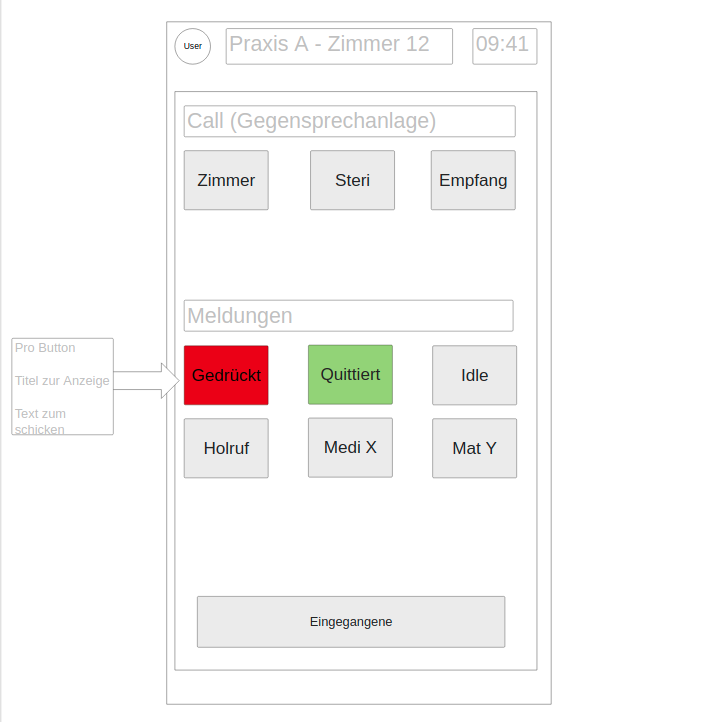
\includegraphics[width=\textwidth]{/home/joshua/FHNW/dev/IP6/IP6_Bachelorarbeit_Bericht_Cloudbasiertes_Praxisrufsystem/src/graphics/mockups/homescreen-mockup}
        \caption{Mockup Home}
    \end{minipage}
    \hfill
    \begin{minipage}[b]{0.4\textwidth}
        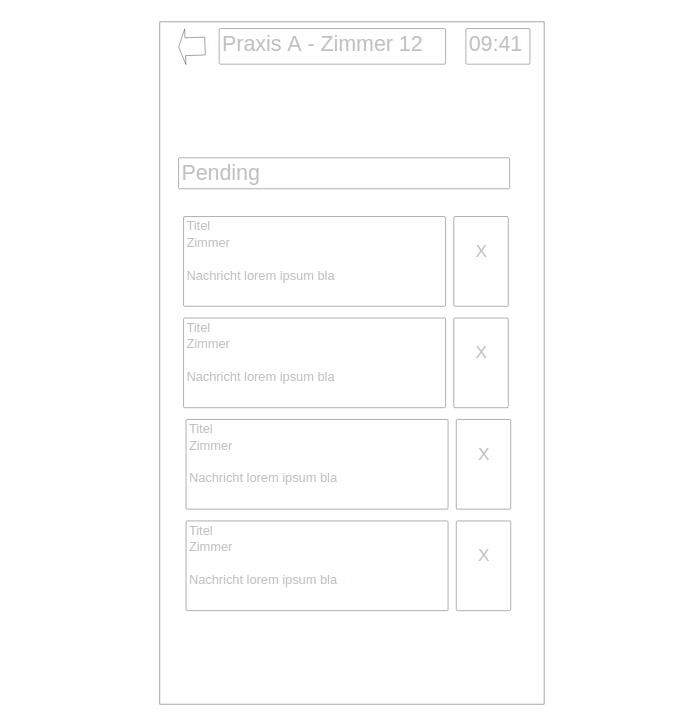
\includegraphics[width=\textwidth]{/home/joshua/FHNW/dev/IP6/IP6_Bachelorarbeit_Bericht_Cloudbasiertes_Praxisrufsystem/src/graphics/mockups/mockup-inbox}
        \caption{Mockup Inbox}
    \end{minipage}\label{fig:HomeScreen-And-Inbox-Mock}
\end{figure}

Active Call Screen \\
Erweiterung Admin UI für Konfiguration CallType \\

\clearpage
\subsubsection*{Konfiguration}

Praxisruf wird um die Funktion einer Gegensprechanlage erweitert.
Dabei soll von einem Administrator zentral konfiguriert werden können, zwischen welchen Clients Sprachverbindungen
aufgebaut werden können.
Damit dies möglich ist, sind Änderungen an der Configuration Domain des Cloud Service von Praxisruf notwendig.

Praxisruf bietet bereits heute die Möglichkeit Buttons zu konfigurieren, über welche Benachrichtigungen versendet werden können.
Diese Buttons werden mit der Entität NotificationType konfiguriert, welche wiederum einer ClientConfiguration zugeordnet werden können.
Diese ClientConfiguration wird bei der Anmeldung auf dem Mobile Client geladen und verwendet um die nötigen Buttons darzustellen.
Analog dazu wird für den Aufbau von Sprachverbindungen eine Entität CallType erstellt.
Diese kann mehreren ClientConfigurations zugeordnet werden.
Ein CallType beinhaltet den Text, welcher auf dem zugehörigen Button auf Clientseite angezeigt wird und eine Liste von
Clients, welche als Ziel der Sprachverbindung verwendet werden.
Es ist möglich, dass dieselbe Gruppe an Zielen auf verschiedenen Clients verschieden heissen soll.
Um dies einfach zu ermöglichen, werden die Ziele der Unterhaltung in eine eigene Entität CallGroup ausgelagert.
So kann pro Client ein CallType definiert werden der einen eigenen Anzeigtext definiert.
Die CallGroup muss aber nur einmal erstellt werden und kann auf mehreren CallTypes verwendet werden.

Die ClientConfiguration die bei der Anmeldung vom Mobile Client geladen wird, wird um diese CallTypes erweitert.
Dabei werden für jeden CallType aber nur der technische Identifikator und der Anzeigename mitgegeben.
Zu welchen Zielen Verbindungen aufgebaut werden sollen, wird bei jedem Verbindungsabbau erneut beim CloudService angefragt.
Dies ermögicht es, dass Änderungen an der Konfiguration sofort angewendet werden, ohne dass die ganze Konfiguration neu geladen werden muss.


\subsubsection*{Verfügbarkeit und Registrierung}

Client muss sich beim Startup beim Signaling Service registrieren.

\clearpage

\subsubsection*{Verbindungsaufbau}

\begin{figure}[h]
    \centering
    \begin{minipage}[b]{0.9\textwidth}
        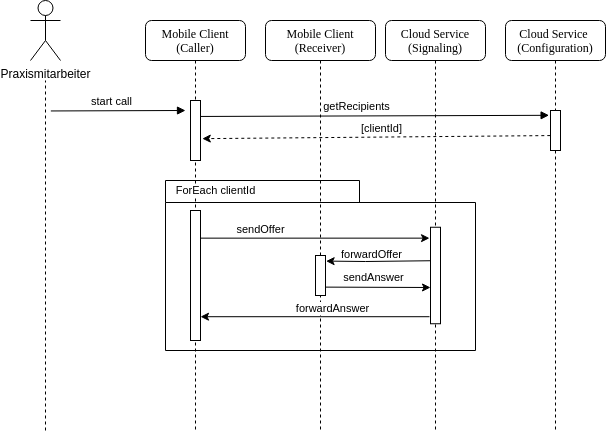
\includegraphics[width=\textwidth]{graphics/diagramms/Sequence_Intercom_Broking_V02}
        \caption{Ablauf Verbindungsaufbau Gegensprechanalge}
    \end{minipage}
\end{figure}



\subsubsection*{Unterhaltung}

Mute Button
End Call Button


\subsubsection*{Verbindungsende}

Caller nimmt Finger vom Button.
Receiver hat button zum abbrechen.

\clearpage
